\chapter{\ifproject%
\ifcpe โครงสร้างและขั้นตอนการทำงาน\else Project Structure and Methodology\fi
\else%
\ifcpe โครงสร้างของโครงงาน\else Project Structure\fi
\fi
}

ในบทนี้จะกล่าวถึงหลักการ และการออกแบบระบบ

\makeatletter

% \renewcommand\section{\@startsection {section}{1}{\z@}%
%                                    {13.5ex \@plus -1ex \@minus -.2ex}%
%                                    {2.3ex \@plus.2ex}%
%                                    {\normalfont\large\bfseries}}

\makeatother
%\vspace{2ex}
% \titleformat{\section}{\normalfont\bfseries}{\thesection}{1em}{}
% \titlespacing*{\section}{0pt}{10ex}{0pt}

\section{ผลการสำรวจของนักศึกเกี่ยวกับตารางสอบปลายภาค}
จากการทำแบบสอบถามเกี่ยวกับตารางสอบปลายภาคของมหาวิทยาลัยชียงใหม่ โดยขอความร่วมมือนักศึกษาที่ทุกระดับชั้นในมหาวิทยาลัยเชียงใหม่ 
ทั้งนักศึกษาที่กำลังศึกษาอยู่และสำเร็จการศึกษาไปแล้ว เพื่อสอบถามความคิดเห็นเกี่ยวกับ ข้อดี ข้อเสีย ของตารางสอบที่แต่ละคนได้รับ 
ร่วมถึงปัญหาที่เคยกระทบมา โดยเราสามารถบอกได้ว่าผู้ทำแบบสอบถามส่วนใหญ่นั้นตรวจสอบดูช่วงเวลาสอบของแต่ละวิชาก่อนที่จะลงทะเบียนอย่างสม่ำเสมอ 
ยังมีผู้ทำแบบสอบถามบางส่วนนั้นตรวจสอบดูช่วงเวลาสอบก่อนจะลงทะเบียนเรียนในบางวิชาไม่สม่ำ และมีผู้ทำแบบสอบถามส่วนน้อยที่ไม่มีเคยตรวจสอบปลายภาคอยู่เลยดังรูปที่ \ref{fig:enroll}
ต่อมาเราได้สอบถามเกี่ยวกับการจัดตารางสอบของสำนักทะเบียนมหาลัยเชียงใหม่ได้ข้อผลสรุปว่าผู้ทำแบบสอบถามส่วนใหญ่นั้นไม่ทราบถึงเวลาการจัดตารางสอบของสำนักทะเบียน มีคนที่ทราบเป็นส่วนน้อยเท่าน้ันที่ทราบถึงวิธีการจัดตารางสอบดังรูปที่ \ref{fig:Create_exam} 
่ต่อมาเราได้สอบถามเวลาที่ผู้ทำแบบสอบถามต้องการจะสอบคือช่วงเวลาใดของสัปดาห์โดยได้ผลลัพธ์ดังรูป\ref{fig:time_slot}โดย 7 ลำดับช่วงเวลาที่ผู้ทำแบบสอบถามอยากสอบมากที่สุดเป็นดังนี้(จากมากไปน้อยตามลำดับ)
\begin{enumerate}
  \item สัปดาห์ที่หนึ่ง เวลา 12.00-15.00น. วันศุกร์ 
  \item สัปดาห์ที่หนึ่ง เวลา 12.00-15.00น. วันจันทร์
  \item สัปดาห์ที่หนึ่ง เวลา 12.00-15.00น. วันพุธ
  \item สัปดาห์ที่สอง เวลา 12.00-15.00น. วันอังคาร
  \item สัปดาห์ที่หนึ่ง เวลา 12.00-15.00น. วันอาทิตย์
  \item สัปดาห์ที่สอง เวลา 12.00-15.00น. วันพฤหัสบดี
  \item สัปดาห์ที่สอง เวลา 12.00-15.00น. วันเสาร์
\end{enumerate}
และเราสามารถสรุปเพิ่มได้ว่าจากการสอบถามเวลาที่ผู้ทำแบบสอบถามต้องการจะสอบนั้นส่วนใหญ่ต้องการที่จะสอบหนึ่งวันเว้นหนึ่งวันเพื่อที่จะได้มีเวลาในการอ่านหนังสือเตรียมสอบสำหรับวิชาในวันต่อไปมากกว่าสอบติดกันและ
ยังสามารถบอกได้อีกว่าผู้ทำแบบสอบถามส่วนใหญ่ต้องการสอบในช่วงสัปดาห์แรกของช่วงการสอบมากกว่าช่วงสัปดาห์สุดของการสอบเพื่อที่จะมีเวลาพักผ่อนหลังจากทำการสอบทั้งหมดดังรูปที่ \ref{fig:day}
และช่วงเวลาที่ผู้ทำแบบสอบถามส่วนใหญ่ต้องการที่จะสอบในแต่ละวันคือช่วงเวลา 12.00-15.00น. ซึ่งผู้ทำแบบสอบถามส่วนมากต้องการจะสอบช่วงเวลานี้มากกว่า 15.30-18.00น. และ 08.00-11.00น. ตามลำดับ
\begin{figure}
\begin{center}
\includegraphics{images/check_enrollment.png}\\[2ex]
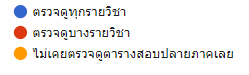
\includegraphics{images/type_check_enrollment.png}
\end{center}
\caption[Poem]{จำนวนนักศึกษาที่ตรวจสอบตารางสอบปลายภาคก่อนการลงทะเบียน}
\label{fig:enroll}     
\end{figure}

\begin{figure}
\begin{center}
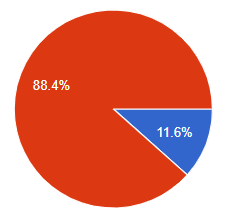
\includegraphics{images/Create_exam.png}\\[2ex]
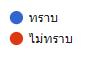
\includegraphics{images/type_Create_exam.png}
\end{center}
\caption[Poem]{จำนวนนักศึกษาที่ทราบวิธีการจัดตารางสอบปลายภาคของสำนักทะเบียน}
\label{fig:Create_exam}     
\end{figure}

\begin{figure}
\begin{center}
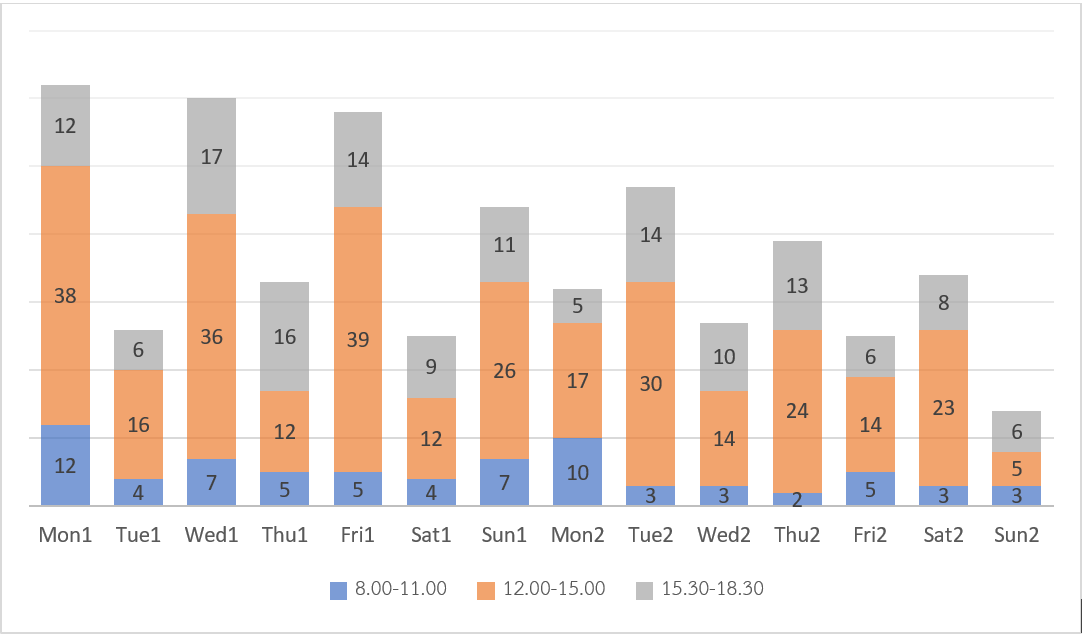
\includegraphics[width=\linewidth]{images/bar_chart.png}
\end{center}
\caption[Poem]{ความต้องการสอบของนักศึกษาในแต่ละช่วงเวลา}
\label{fig:time_slot}     
\end{figure}

\begin{figure}
\begin{center}
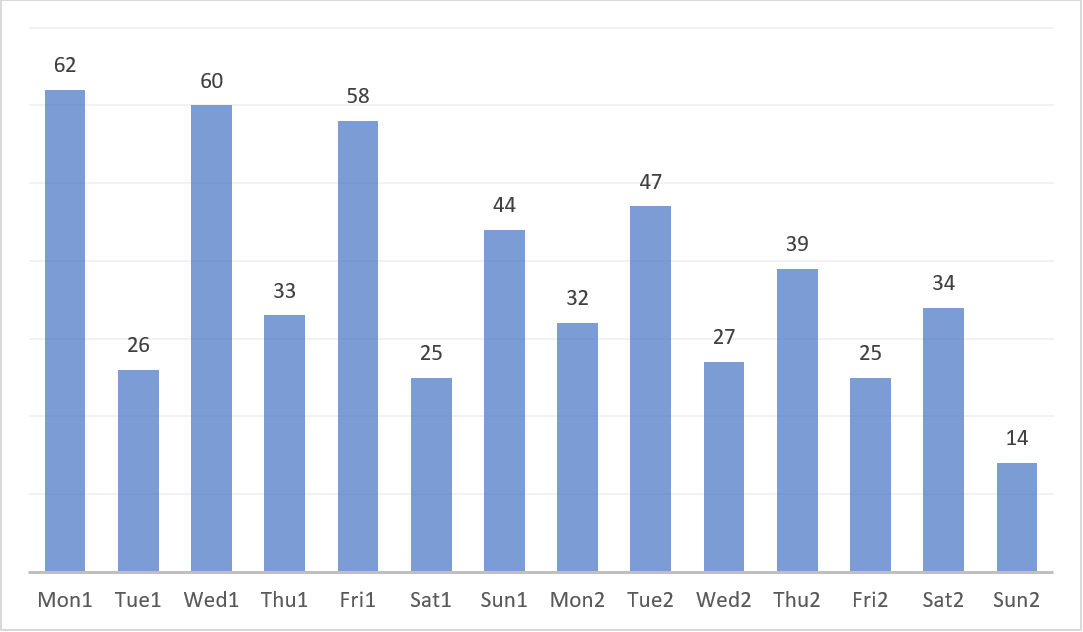
\includegraphics[width=\linewidth]{images/chart.png}
\end{center}
\caption[Poem]{ความต้องการสอบของนักศึกษาในแต่ละวัน}
\label{fig:day}     
\end{figure}

\begin{figure}
\begin{center}
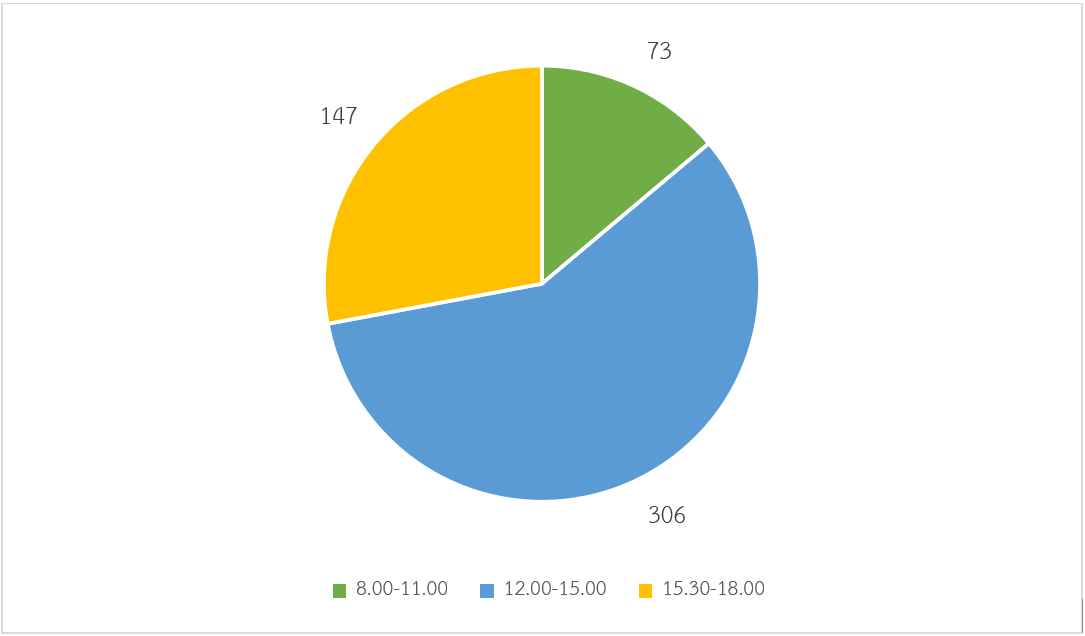
\includegraphics[width=\linewidth]{images/pie.png}
\end{center}
\caption[Poem]{ความต้องการสอบของนักศึกษาในแต่ละวเวลา}
\label{fig:time}     
\end{figure}


